\begin{flushright}
    \textit{Лекция 9 (от 05.10)}
\end{flushright}
\corollary
~
\begin{enumerate}
    \item $a \neq \infty$~--- полюс $f$ $\Leftrightarrow$ $\exists
    \overset{\circ}{B}_{\rho}(a), \ \exists m \in \NN, \ \exists p: B_{\rho}(a)
    \mapsto \CC$~--- регулярная, причем $p(a) \neq 0$, для которой верно:
    \begin{equation}\label{(12.3)}
        f(z) = \frac{p(z)}{(z-a)^m} \ \forall z \in \overset{\circ}{B}_\rho(a)
    \end{equation}
    \item $a = \infty$~--- полюс $f$ $\Leftrightarrow$ $\exists
    \overset{\circ}{B}_{\rho}(\infty), \ \exists m \in \NN, \ \exists h:
    B_{\rho}(\infty) \mapsto \CC$~--- регулярная, причем $\dst\lim_{z \to
      \infty} h(z) = h(\infty) \neq 0$, для которой верно:
    \begin{equation}\label{(12.4)}
        f(z) = z^mh(z) \ \forall z \in \overset{\circ}{B}_\rho(\infty)
    \end{equation}
\end{enumerate}
\Def \label{[12.3]}
Пусть $a$~--- полюс $f$, $m$ определено из \eqref{(12.3)} или
\eqref{(12.4)}. Тогда $m$ называется \textbf{порядком полюса $a$}.
\Def \label{[12.4]}
Пусть $g: B_R(a) \mapsto \CC$ регулярна, и $g(a) = g'(a) = \dots = g^{(n-1)}(a)
= 0$, $g^{(n)}(a)\neq 0$. Тогда $a$ называется \textbf{нулем $n$-го порядка
  функции $g$}.
\corollary
Пусть $g$, $h: B_\rho(a) \mapsto \CC$ регулярны; пусть $a$~--- нуль $k$-го
порядка функции $g$, причем $k \geq 0$, и $m$-го порядка функции $h$, причем $m
\geq 1$. Тогда для $f = \dst \frac{g}{h}$ точка $a$ будет:
\begin{enumerate}
    \item полюсом $(m-k)$-го порядка, если $m > k$;
    \item УОТ, если $m \leq k$.
\end{enumerate}
\pr
По определению \ref{[12.4]}
\begin{align*}
  & g(z) = (z-a)^kg_1(z), \ g_1(a) \neq 0
\end{align*}
\begin{align*}
  & g(z) = (z-a)^mh_1(z), \ h_1(a) \neq 0
\end{align*}
Тогда
\begin{align*}
  & p(z) = \frac{g_1(z)}{h_1(z)}
\end{align*}
регулярна в некоторой окрестности $a$, $p(a) \neq 0$. Тогда из следствия $1$
получаем желаемое.
\note
Существуют неизолированные особые точки. Пусть
\begin{align*}
  & f(z) = \frac{1}{\sin \frac{\pi}{z}}
\end{align*}
Тогда $z_n = \dst \frac{1}{n}$~--- особые точки, но $0$~---
неизолированная особая точка (предельная точка полюсов).
\Exse
Пусть $a$~--- полюс $f$ и существенно особая точка $g$. Чем является $a$ для $h
= fg$?
\Exse
Пусть $a$~--- полюс $f$. Чем является $a$ для $g= f^2$?
\Exse
Пусть $a$~--- существенно особая точка $f$. Чем является $a$ для $g = \dst
\frac{1}{f}$?
\Exse
Пусть $a$~--- полюс $f$. Чем является $a$ для $g = e^f$?
\section{$\S 13.$ Теория вычетов}
\Def
Пусть $a \in \CC$~--- ИОТ $f: \overset{\circ}{B}_\rho(a) \mapsto \CC$. Тогда
\textbf{вычетом $f$ в точке $a$} называется
\begin{equation}\label{(13.1)}
    \us{a}{\res}f = \frac{1}{2\pi i}\int_{\gamma_r}f(z)dz
\end{equation}
где $\gamma_r = \sets{z \mid \abs{z-a} = r}$ положительно ориентирована, $r \in
(0; \rho)$.
\\
\property
$f$ регулярна в $\os{\circ}{B}_\rho(a)$ $\Rightarrow$ существует ряд Лорана с
центром в точке $a$, причем
\begin{equation}\label{(13.2)}
    \begin{split}
        & c_n = \frac{1}{2 \pi i}\int_{\gamma_r}\frac{f(\zeta)}{(\zeta - a)^{n+1}}d \zeta \\
        & \us{a}{\res}f = c_{-1}
    \end{split}
\end{equation}
\lemma
Пусть $a$~--- полюс $m$-го порядка функции $f$. Тогда
\begin{equation}\label{(13.3)}
    \us{a}{\res} f = \frac{1}{(m-1)!}\lim_{z \to a}\frac{d^{m-1}}{dz^{m-1}} \left( (z-a)^mf(z) \right)
\end{equation}
\pr
\begin{align*}
  & f(z) = \frac{c_{-m}}{(z-a)^m} + \dots + \frac{c_{-1}}{z-a} + c_0 + c_1(z-a) + \dots
\end{align*}
\begin{align*}
  & (z-a)^mf(z) = c_{-m}+ c_{-m+1}(z-a) + \dots + c_{-1}(z-a)^{m-1} + \dots
\end{align*}
По теореме Вейерштрасса можно дифференцировать ряд:
\begin{align*}
  & \frac{d^{m-1}}{dz^{m-1}}\left( (z-a)^mf(z)\right) = (m-1)!c_{-1} + m!c_0(z-a) + \dots
\end{align*}
Переходя к пределу $z \to a$, получаем \eqref{(13.3)}.
\lemma
Пусть $f(z) = \dst \frac{P(z)}{Q(z)}$, $P(z)$, $Q(z)$ регулярны в $B_\rho(a)$ и
$P(a) \neq 0$, $Q(a) = 0$, $Q'(a) \neq 0$. Тогда
\begin{equation}\label{(13.4)}
    \us{a}{\res} f = \frac{P(z)}{Q'(z)}
\end{equation}
\pr
Из \eqref{(13.3)} получаем:
\begin{align*}
  & \us{a}{\res}f = \lim_{z\to a}\left( (z-a)\frac{P(z)}{Q(z)} \right) = \lim_{z \to a} \frac{P(z)}{\left( \frac{Q(z) - Q(a)}{z-a} \right)}
\end{align*}
что, по определению производной, равносильно \eqref{(13.4)}.
\Def
Пусть $\infty$~--- ИОТ $f: \os{\circ}{B}_{R_0}(\infty) \mapsto \CC$, тогда
\begin{equation}\label{(13.5)}
    \us{\infty}{\res}f = \frac{1}{2\pi i}\int_{\gamma_R^{-1}}f(z)dz
\end{equation}
где $\gamma_R = \sets{z \mid \abs{z} = R}$ положительно ориентирована, $R >
R_0$.
\lemma
Пусть $\infty$~--- УОТ $f$; тогда
\begin{equation}\label{(13.6)}
    \us{\infty}{\res}f = \lim_{z \to \infty} \left( z(f(\infty) - f(z)) \right)
\end{equation}
\pr
\begin{align*}
  & f(z) = f(\infty) + \frac{c_{-1}}{z} + \frac{c_{-2}}{z^2} + \dots
\end{align*}
\begin{align*}
  & z(f(\infty) - f(z)) = -c_{-1} - \frac{c_{-2}}{z} - \dots
\end{align*}
Устремляя $z \to \infty$, получаем \eqref{(13.6)}.
\theorem (Коши о вычетах)
Пусть $G \subseteq \CCC$~--- область с положительно ориентированной кусочно
гладкой границей $\Gamma$. Пусть $\ol{G} = G \cup \Gamma$.
\\
Пусть $g: \ol{G} \mapsto \CC$ регулярна в $G$ за исключением конечного числа ИОТ
$a_1, \dots, a_n$, причем если $\infty \in \ol{G}$, то $a_n = \infty$, и
непрерывна на $\ol{G}\setminus \left( \dst \bigcup_{k=1}^n\{a_k\} \right)$.
Тогда
\begin{equation}\label{(13.7)}
    \int_{\Gamma}f(z)dz = 2 \pi i \sum_{k=1}^{n}\us{a_k}{\res} f
\end{equation}
\pr
~
\begin{enumerate}
    \item Рассмотрим случай: $G$ ограничена, $\exists r > 0:$ окрестности
    $\ol{B_r(a_k)}\subseteq G$ и не пересекаются.
    \\
    Пусть $\gamma_k = \{\zeta \mid \abs{\zeta - a_k} = r\}$ положительно
    ориентированы.
    \\
    Пусть
    \begin{align*}
      & \tilde{G} = G \setminus \left( \bigcup_{k=1}^n\ol{B_r(a_k)} \right)
    \end{align*}
    \begin{align*}
      & \tilde{\Gamma} = \Gamma \cup \left( \bigcup_{k=1}^n  \gamma_k^{-1} \right)
    \end{align*}
    Тогда по теореме $3$ $\S7$
    \begin{align*}
      & 0 = \int_{\tilde{\Gamma}}f(z)dz =  \int_{\Gamma}f(z)dz + \sum_{k=1}^n\int_{\gamma_k^{-1}}f(z)dz =  \int_{\Gamma}f(z)dz -2 \pi i \sum_{k=1}^n\us{a_k}{\res}f(z)
    \end{align*}
    \item Рассмотрим второй случай: $\infty \in G$, $a_n = \infty$, $\Gamma$
    ограничена.
    \\
    Тогда
    \begin{align*}
      & \exists R_0 > 0: \ \forall z \in \Gamma \cup \left( \bigcup_{k=1}^{n-1}\{a_k\} \right) \abs{z} < R_0
    \end{align*}
    \\
    Тогда 
    \begin{align*}
      & \forall R > R_0: \ \tilde{G} = G \cap B_R(0), \ \tilde{\Gamma} = \Gamma \cup \gamma_R
    \end{align*}
    $\gamma_R = \{z \mid \abs{z} = R\}$~--- положительно ориентирована.
    Тогда из пункта $1$
    \begin{align*}
      & \int_{\tilde{\Gamma}}f(z)dz = 2 i \pi \sum_{k=1}^{n-1}\us{a_k}{\res}f(z) =  \int_{\Gamma}f(z)dz +  \int_{\gamma_R}f(z)dz =  \int_{\Gamma}f(z)dz - 2 \pi i \us{\infty}{\res} f
    \end{align*}
\end{enumerate}
\corollary
Пусть $f$ регулярна в $\CC$ за исклчением конечного числа ИОТ $a_1, \dots, a_n$
($a_n = \infty$). Тогда
\begin{equation}\label{(13.8)}
    \sum_{k=1}^n\us{a_k}{\res}f = 0
\end{equation}
\pr
\begin{align*}
  & \exists R_0: \ \forall k \in \{1, \dots, n-1\} \ \abs{a_k} \leq R_0
\end{align*}
Пусть $\gamma_{R_0} = \{z \mid \abs{z} = R_0\}$ положительно ориентирована.
\\
Тогда
\begin{align*}
  & \int_{\gamma_{R_0}}f(z)dz = 2 \pi i \sum_{k=1}^{n-1} \us{a_k}{\res}f
\end{align*}
\begin{align*}
  & \int_{\gamma_{R_0}}f(z)dz = -2 \pi i \us{\infty}{\res}f
\end{align*}
Отсюда очевидно следует \eqref{(13.8)}.
\Example
\begin{align*}
  & I = \int_{\abs{z} = 3}\frac{z dz}{(z-1)(z-2)}
\end{align*}
Особые точки~--- $z=1$, $z=2$~--- полюса $1$ порядка.
\\
По теореме Коши о вычетах ($13.1$)
\begin{align*}
  & I = 2 \pi i \left( \us{1}{\res} \frac{z}{(z-1)(z-2)} +  \us{2}{\res} \frac{z}{(z-1)(z-2)}\right) = 2 \pi i \left( \left. \frac{\left( \frac{z}{z-2} \right)}{(z-1)'} \right|_{z=1} +  \left. \frac{\left( \frac{z}{z-1} \right)}{(z-2)'} \right|_{z=2} \right) = 2 \pi i
\end{align*}
\Example
\begin{align*}
  & I = \int_{-\infty}^{+\infty}\frac{1+x^2}{1+x^4}dx
\end{align*}
Продолжим на комплексную плоскость:
\begin{align*}
  & f(z) = \frac{1+z^2}{1+z^4}
\end{align*}
Особые точки: $z_k = \exp \left( i \left( \dst \frac{\pi}{4} + \dst \frac{\pi
          k}{2} \right) \right), \ k \in\{0, 1, 2, 3\}$.
\\
Положим $\gamma_R = \left[ -R;R \right] \cup \{z \mid \abs{z} = R, \ \Img z \geq
0 \} = \left[ -R;R \right] \cup C_R$.
\begin{figure}[h!]
		\centering
		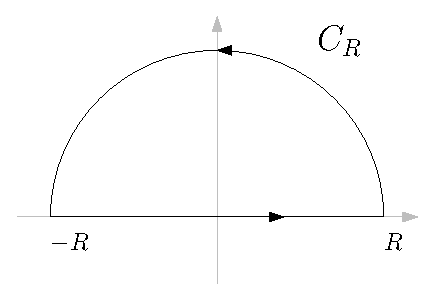
\includegraphics[scale=1]{circ.eps}
    \caption{Полукруг в верхней полуплоскости с обходом против часовой стрелки}
		\label{fig:13.1}
\end{figure}
\\
Пусть 
\begin{align*}
  & I_R = \int_{\gamma_R}f(z)dz = 2 \pi i \left( \us{z_0}{\res} f(z) +  \us{z_1}{\res} f(z)\right) = 2 \pi i \left( \left.\frac{1+z^2}{4z^3}\right|_{z_0} + \left.\frac{1+z^2}{4z^3}\right|_{z_1}\right) = 2 \pi i \cdot \\
  & \cdot \left( \frac{1+\exp\left( \frac{2i \pi}{4} \right)}{4 \exp \left( \frac{3i \pi}{4} \right)} +  \frac{1+\exp\left( \frac{6i \pi}{4} \right)}{4 \exp \left( \frac{9i \pi}{4} \right)}\right) = 2 \pi i \left( \frac{\exp\left( \frac{-i\pi}{4} \right) + \exp\left( \frac{i\pi}{4} \right)}{2 i \cdot 2} +  \frac{\exp\left( \frac{-3i\pi}{4} \right) + \exp\left( \frac{3i\pi}{4} \right)}{-2 i \cdot 2}\right) = \\
  & = \pi \left( \cos \frac{\pi}{4} - \cos \frac{3\pi}{4} \right) = \pi \sqrt{2}
\end{align*}
\begin{align*}
  & \pi \sqrt{2} = \int_{-R}^{+R}f(z) + \int_{C_R}f(z) \us{R\to \infty}{\longrightarrow} \int_{-\infty}^{+\infty} f(z) = \int_{-\infty}^{\infty}f(x)
\end{align*}
Итак, достаточно доказать
\begin{align*}
  & \int_{C_R}f(z)  \us{R\to \infty}{\longrightarrow} 0
\end{align*}
чтобы получить, что $I = \pi \sqrt{2}$.